\chapter{Systemmodelle}

\section{MVVM-Architektur}
\setcounter{counterKriterien}{0}

Es wird die MVVM-Architektur zur Realisierung von \projektTitel verwendet.

\nItem{S} Model \\
Hier befinden sich die unter Produktdatenaufgeführten punkte , Filter sowie Analysemetriken. Wenn die Daten
sich ändern schickt das Model eine Benachrichtigung an sein ViewModel.

\nItem{S} ViewModel \\
Im ViewModel werden alle vom Benutzer erhaltenen Eingaben entsprechend verarbeitet und
gegebenenfalls an das Model weitergeleitet, es leitet auch die Daten des Models and das View weiter.

\nItem{S} View \\
Ein View ist die Präsentation der Daten des Models. In unserem Fall zeigt unsere Gui den aktuellen Zusatnd des Modells.


\section{Szenarien}
% Nutzt bitte dieses template für neue Szenarien
% Haltet ein Szenario bitte kürzer als eine Seite (kompilieren-> prüfen), sonst
% läuft es über die Fußzeile hinaus. Man kann es zwar mit longtable umgehen
% aber die Ereignissflussspalte wird dann auf einer eigenen Seite gedruckt.
% Außerdem sollte ein Szenario nicht so lang sein :-).
%\begin{tabular}{p{1.55cm}|p{14cm}}
%Szenario-Name & \\ \hline
%Akteur-Instanzen & \\ \hline
%Ereignis-fluss & \begin{compactenum}[1]
%\item 
%\end{compactenum} \\
%\end{tabular}


\begin{tabular}{p{1.55cm}|p{14cm}}
Szenario-Name & Scharfzeichner-Analyse\\ \hline
Akteur-Instanzen &Bob:VideoEncoderEntwickler\\ \hline
Ereignis-Fluss & \begin{compactenum}[1]
\item Bob startet \projektTitel, es erscheint ein Willkomensfenster auf dem allgemeine Informationen und seine zuletzt geöffneten Projekte angezeigt werden.
\item Bob klickt auf das ">Projekt erstellen"< Symbol aus der Werkzeugleiste.
\item Es öffnet sich ein ">Neues Projekt"< Assistent, in dem Bob ein Referenzvideo im \gls{glos:YUV} Format einträgt.
\item Bob überprüft die eingegebenen Informationen und klickt auf den ">Projekt erstellen"< Button. Das neue Projekt wird geöffnet.
\item Bob wählt das von ihm zuvor angegebene Video aus dem Projektexplorer.
\item Bob wählt den Weichzeichner-Filter aus dem Filterkatalog-Tab. Im Filter-Paramter-Abschnitt stellt er die Intensität des Weichzeichner-Effekts ein und klickt anschließend auf das ">Filter anwenden"< Symbol aus der Werkzeugleiste 
\item Bob minimiert nun \projektTitel und öffnet sein zu testendes Scharfzeichner-Werkzeug auf dem gerade durch den Weichzeichner-Filter generierten Testvideo, das neu im Projektordner erstellt wurde.
\item Bob wechselt nun wieder zu \projektTitel. Er wählt in der Werkzeugleiste die Option ">Testvideo hinzufügen"< und lädt das gerade durch sein Scharfzeichner-Werkzeug erstellte Video in sein Projekt.
\item Bob wählt das ursprüngliche Referenzvideo ohne Weichzeichner-Effekt und sein gerade vom Scharfzeichner bearbeitetes Video an, um diese zu vergleichen.
\item Dazu klickt Bob auf das ">Metriken"<-Tab. Anstelle des Filterkatalogs sieht er nun eine Auswahl an Analysemetriken. Bob doppelklickt auf den Eintrag \gls{MSE}.
\item Der Eintrag \gls{MSE} ist nun hervorgehoben. Bob klickt auf das ">Analyse"< Symbol aus der Werkzeugleiste.
\item Im Log-Fenster wird nun zusätzlich zu den aktuellen Statusmeldungen ein Fortschrittsbalken angezeigt. Bob wartet bis der Vorgang beendet ist.
\item Nach Abschluss des Analysedurchlaufs werden Bob die Ergebnisse der Analyse im Hauptfenster von \projektTitel graphisch dargestellt.
\item Bob weiß nun, dass sein Scharfzeichner-Werkzeug den Weichzeichnungseffekt nur mangelhaft beseitigen konnte. Das neu gewonnenen Wissen nutzt er um sein Werkzeug zu verbessern.
\end{compactenum}\\
\end{tabular}
%-------------------------------------------------------------------------------------------------------
\section{Anwendungsfälle}

\begin{figure}[h]
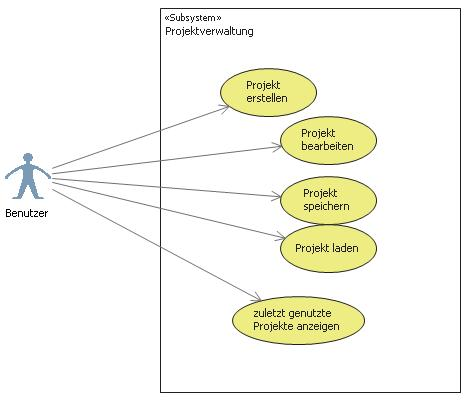
\includegraphics[scale=1]{bilder/anwendungsfalldiagramm_projektverwaltung.jpg}
\label{Anwendungsfalldiagramm_Projektverwaltung}
\caption{Anwendungsfall-Diagramm der Projektverwaltungs-Funktionalitäten}
\end{figure}

\begin{figure}[h]
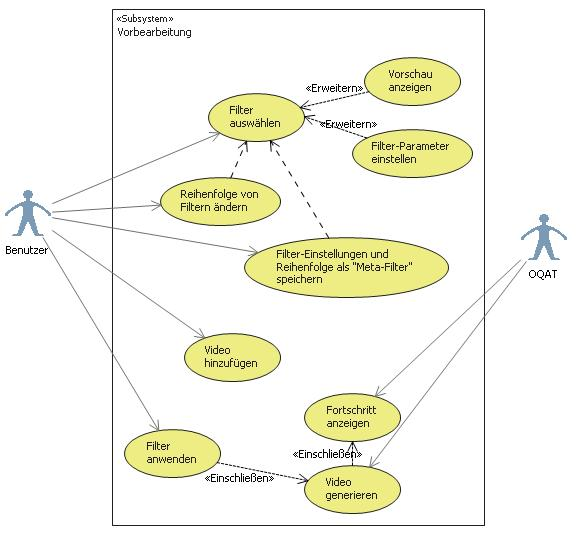
\includegraphics[scale=1]{bilder/anwendungsfalldiagramm_filter.jpg}
\label{Anwendungsfalldiagramm_Filter}
\caption{Anwendungsfall-Diagramm der Filter-Funktionalitäten}
\end{figure}

\begin{figure}[h]
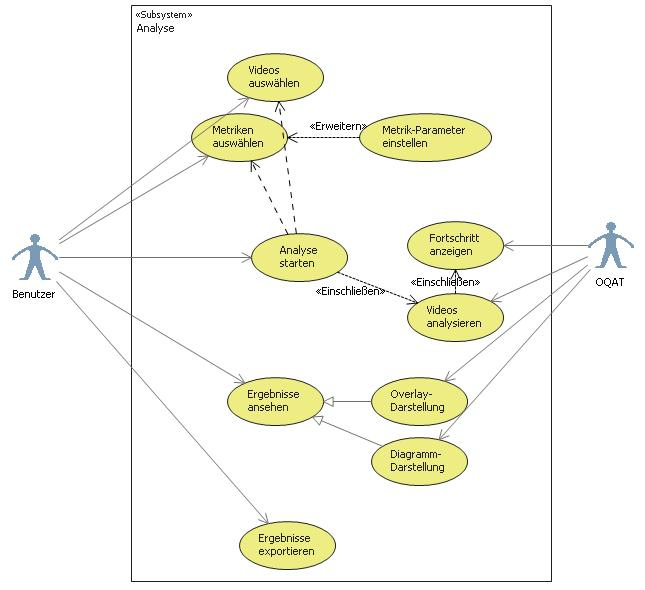
\includegraphics[scale=1]{bilder/anwendungsfalldiagramm_analyse.jpg}
\label{Anwendungsfalldiagramm_Analyse}
\caption{Anwendungsfall-Diagramm der Analyse-Funktionalitäten}
\end{figure}


% template für Anwendungsfälle, gleiche Vorschläge wie für szenario.
% Beachtet richtlinien für Anwendungsfälle (tichy oder bruegge)
%\begin{tabular}{p{2.2cm}|p{13cm}} \hline
%Anwendungs-fallname & someName\\ \hline
%Akteur & SomeActor\\ \hline
%
%Ereignisfluss & \begin{compactenum}
%\item Some process.
%\end{compactenum}\\ \hline
%
%Anfangs-bedingungen & \begin{compactitem}
%\item Some point.
%\end{compactitem} \\ \hline
%
%Abschluss-bedingungen & \begin{compactitem}
%\item Some point
%\end{compactitem}\\ \hline
%
%Qualitäts-anforderungen & \begin{compactitem}
%\item Some point
%\end{compactitem}\\ \hline
%
%\end{tabular}

%-------------------------------------------------------------------------------------------------------
\section{Objektmodell}
%-------------------------------------------------------------------------------------------------------
\section{Dynamische Modelle}
%-------------------------------------------------------------------------------------------------------
\section{Grafische Benutzerschnittstelle}